\chapter{适应未知背景的可微分逆渲染方法}
\label{chap:method}

在重建3D人脸几何形状时,现有方法未能充分利用照片中的边缘信息。
它们大多依赖2D人脸关键点识别的结果来监督几何形状的优化,但这需要额外的标注步骤,且会引入累计误差,稀疏的关键点信息也会限制优化的精度。
也有方法利用传统的多目立体方法来确定几何形状,但这限制了其必须使用多视角照片作为输入。

很多现有方法也运用了可微分渲染技术,但未能充分利用可见性梯度。
而该梯度正是所有梯度中的主要分量,对模型与照片中边缘的精确对齐有着重要作用。
然而,计算正确的可见性梯度需要同时具有前景和背景的模型,但在自然环境照片中,由于背景多样,很难得到准确的背景模型。
本章主要针对该问题,提出一种适应未知背景的可微分渲染方法,能够利用可见性梯度来优化模型,使其与照片中边缘对齐。

\section{问题定义}

可微分渲染旨在从参数化的3D模型,如三角形面片,纹理贴图等,渲染得到2D图片,同时计算该渲染结果关于其输入参数的梯度。
然后可以优化渲染结果与照片间的误差,以期利用基于梯度的方法优化输入参数,从而改善渲染效果,使之更加接近现实。
其在3D人脸重建的相关任务中已有较广泛的应用。

然而现有方法存在一些不足:
现有可微分渲染技术大多是对整张图片估计梯度,即不区分前景和背景部分。
但是,在基于自然环境照片的人脸重建任务中,我们通常只有前景(即人脸)的3D模型,而没有背景的模型。
此时,现有方法选择忽略模型间相互遮挡产生的可见性梯度,而这会造成模型与照片的对齐不准确,如图\ref{fig:problem_a}所示。
另一方面,若对背景进行很粗糙的建模,例如假设为全黑,则错误的梯度会导致模型无法正确收敛,如图\ref{fig:problem_b}所示。

\begin{figure}
\centering
\begin{subfigure}[t]{0.5\textwidth}
    \centering
    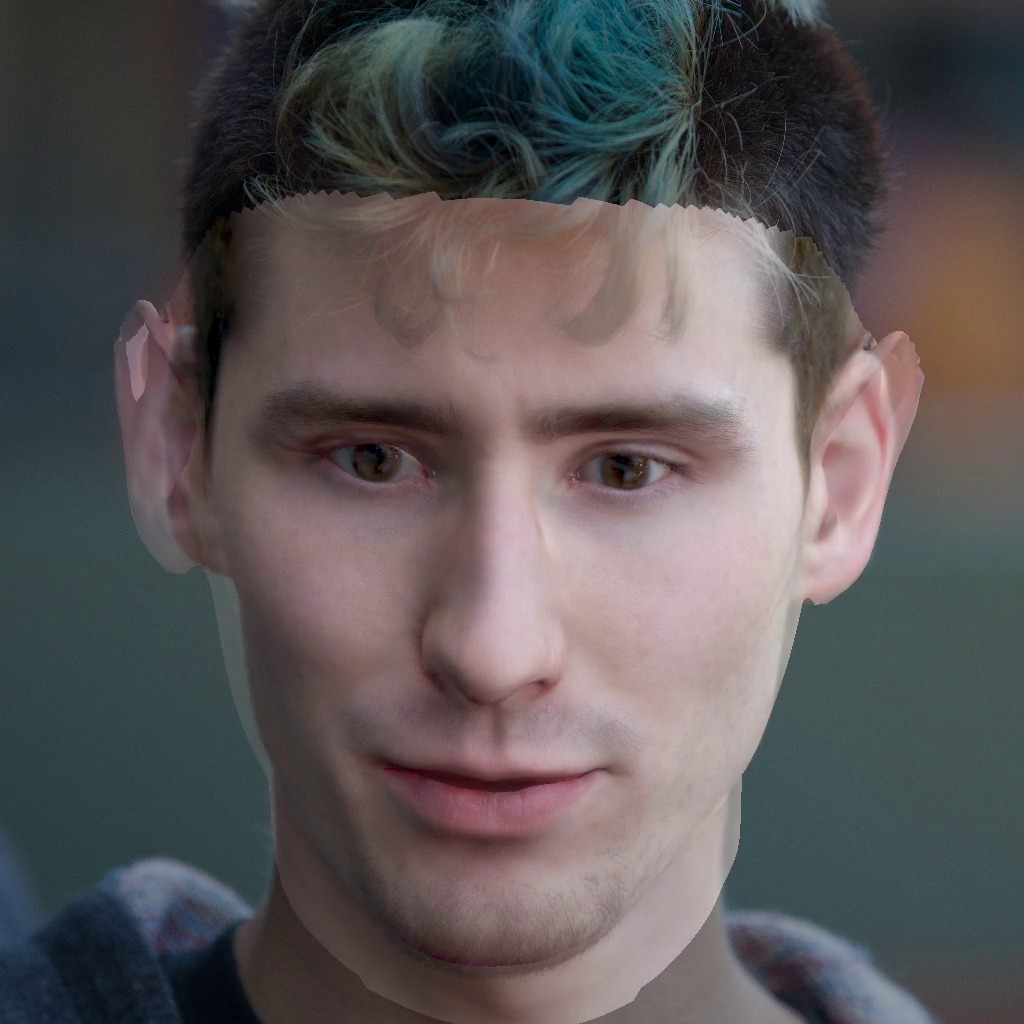
\includegraphics[width=0.8\textwidth]{figures/black-bg_no-aa}
    \caption{忽略可见性梯度,模型与照片未准确对齐}
    \label{fig:problem_a}
\end{subfigure}%
\begin{subfigure}[t]{0.5\textwidth}
    \centering
    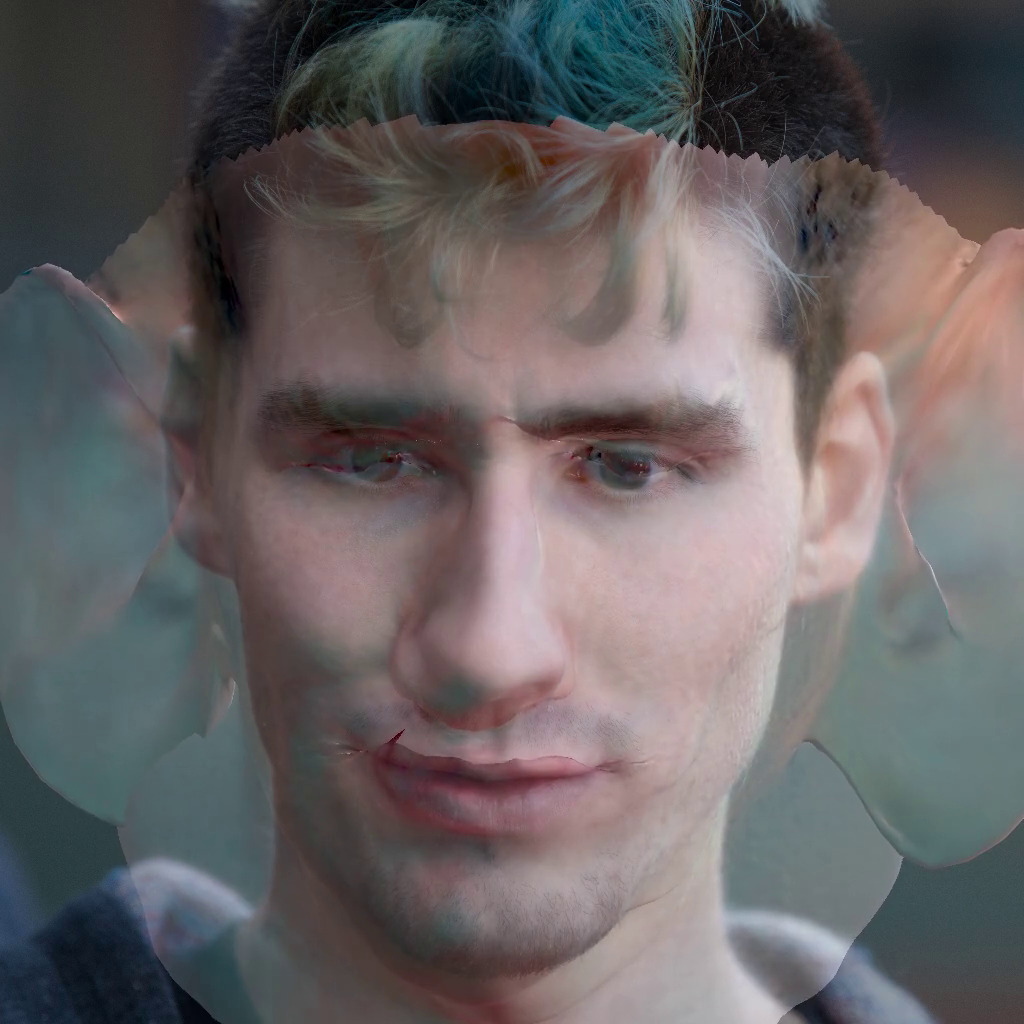
\includegraphics[width=0.8\textwidth]{figures/black-bg}
    \caption{使用全黑代替背景模型,可见性梯度错误}
    \label{fig:problem_b}
\end{subfigure}%
\caption[未知背景条件下可微分渲染优化结果]{
    未知背景条件下可微分渲染优化结果。
    示意图为渲染结果叠加在目标照片上。
}
\end{figure}

为绕过上述问题,现有方法通常:
使用多目立体等其他手段事先确定高精度的人脸几何形状,并在逆渲染优化过程中使几何形状保持不变\citep{RiviereGBGB20};
忽略可见性梯度,使用2D人脸关键点\citep{deep3d}、图像分割\citep{nvdiffrec}结果等辅助监督信息来补足这部分缺失的梯度。
但是,如果能够直接利用可见性梯度,可大大简化算法的流程,同时也能避免在前序步骤中引入额外的误差。

\begin{figure}
    \centering
    \import{build/figures/}{problem.pgf}
    \caption[在未知背景时计算可见性梯度困难]{
        在未知背景时计算可见性梯度困难。
        拟合目标(第一行)和渲染结果(第二行)左侧白色为前景,右侧为背景。
        在第二行中,前景模型为以红线为边界的白色平面。
        横坐标为前景模型的平移量。
        函数值为每像素均匀采样65536次的数值近似。
        (a)离散采样,不计算可见性梯度;
        (b)使用不准确的黑色背景模型计算可见性梯度,模型无法收敛到期望位置;
        (c)理想情况下,在完全已知背景时的可见性梯度,模型能准确收敛至梯度为0的点。
    }
    \label{fig:problem}
\end{figure}
本节将设计一个简单的玩具实验来更直观地说明上述问题。
如图\ref{fig:problem}所示,我们使用一个简单的白色平面作为前景模型,用其拟合一个白色青色对半分割的场景。
该模型的参数是其横向的平移量,用平面边缘与横坐标轴的交点$a_x$表示。
该平面的边缘稍微倾斜,以突出可见性梯度的变化。
该平面的着色不受参数影响,始终固定为白色。
该例子中使用的损失函数为L1误差,即:
\begin{equation}
\mathcal{L} = \left\| \hat{\mathcal{I}} - \mathcal{I} \right\|_1
\text{。}
\label{eq:loss_l1}
\end{equation}

在该实验中,(a)为离散采样的方式,也是目前大多人脸重建中使用的方法。
其渲染流程为:在每个像素的中点处采样,若其位于前景模型的覆盖范围内,则渲染为白色,否则渲染为背景。
由于采样过程是离散的,且$a_x$的改变并不会影响采样的模式,因此,渲染结果$\hat{\mathcal{I}}$关于$a_x$的梯度为0,其损失函数为阶梯函数。
即该损失函数完全无法以基于梯度的方式指导模型拟合。

另一方面,在没有准确背景模型的前提下,可见性梯度则难以被利用。
例如,在(b)中,假设我们并不知道该场景的背景,因此直接假设其为全黑。
但在本例中这个假设显然是不准确的。
(b)和(c)的渲染方式与(a)不同,其每个像素的颜色取决于前景模型覆盖该像素的面积的比例,并按面积比例线性混合前景和背景的颜色。
这使得处于前景边缘处的像素的颜色成为了关于$a_x$的连续函数,即产生了所谓的可见性梯度。
在此前提下,从图中可以观察到其损失函数呈递减的趋势,并未在期望的位置上形成极值。
因此,该梯度也无法引导模型收敛到期望的位置。

作为参考,(c)展示了理想中,完全已知背景的情况下,可见性梯度的作用。
从图中可见,其损失函数在期望的位置上有一个明显的极值,且其周围的梯度将能很好地指导优化器,使模型收敛到该位置。

然而,在实际人脸重建的任务中,特别是从自然环境照片的重建中,背景可能是很复杂且难以建模的。
本章将探讨如何在这种情况下,如何利用可见性梯度以指导前景模型与目标照片对齐。

\section{面积归一化的像素损失函数}

在分析中,不妨先将目标照片$\hat{\mathcal{I}}$和渲染结果$\mathcal{I}$抽象为连续的颜色场$\mathbb{R}^2 \to \mathbb{R}^3$。
于是公式\ref{eq:loss_l1}中的原始L1损失函数可改写为:
\begin{equation}
\mathcal{L} = \iint_{\mathcal{A}} \left\| \hat{\mathcal{I}} - \mathcal{I} \right\|_1 \mathrm{d}\sigma +
\iint_{\mathcal{B}} \left\| \hat{\mathcal{I}} - \mathcal{I} \right\|_1 \mathrm{d}\sigma
\text{,}
\label{eq:loss_l1_area}
\end{equation}
其中,$\mathcal{A}$为渲染结果中前景模型覆盖的区域,$\mathcal{B}$为背景覆盖的区域。
由此我们可以对图\ref{fig:problem}b中的现象进一步地解释:
当前景模型的边界向右移动越过中点之后,由于不能很好地拟合背景,该损失函数的第一项开始上升,这是符合预期的。
但是,由于采用的背景模型不准确,背景部分也存在一定误差,且由于背景区域面积下降,损失函数的第二项将会下降。
这两项相互制衡,导致前景和背景模型“抢夺”处于交界处的像素。
若背景模型的误差足够大,以至于使用前景模型来拟合背景区域反而占优势,则会出现如(b)中的现象:前景模型将在优化中不断抢占背景的区域,从而无法收敛到期望的位置。
在实际中这种情况是很有可能的,比如在3D人脸重建中,人脸的材质模型通常具有很高的自由度以拟合人脸的细节,这些自由度可能被误用于拟合背景。

为解决在未知背景下的逆渲染问题,本文提出了一种面积归一化的像素损失函数:
\begin{equation}
\mathcal{L}_n = \frac{\iint_{\mathcal{A}} \left\| \hat{\mathcal{I}} - \mathcal{I} \right\|_1 \mathrm{d}\sigma}
{\iint_{\mathcal{A}}\mathrm{d}\sigma}
-\alpha\iint_{\mathcal{A}}\mathrm{d}\sigma
\text{。}
\label{eq:loss_n}
\end{equation}
该损失函数仅在前景模型覆盖的区域内计算损失,因此不会受到背景模型的误差影响。
该函数第一项为单位前景区域面积内的平均误差,第二项鼓励更大的前景区域,$\alpha$为一个超参数。

\begin{figure}
\centering
\import{build/figures/}{one_dim_loss.pgf}
\caption{面积归一化的像素损失函数在一维的作用分析}
\label{fig:one_dim_loss}
\end{figure}

为了更好地理解该损失函数的作用,本文将展示一个一维情况下的简单例子。
如图\ref{fig:one_dim_loss}a所示,假设拟合目标包含前景和背景,为阶跃函数;前景模型为定义在前景区域$\mathcal{A}=(0,\theta)$的常函数,$\theta$为模型参数:
\begin{align}
\mathcal{I}(x) &= \begin{cases}
    1   & x \leq 0.6 \\
    0.1 & x > 0.6
\end{cases}\\
\hat{\mathcal{I}}(x) &= 0.8 \quad x < \theta
\text{。}
\end{align}
在此定义下,我们可求出$\mathcal{L}_n(\theta)$中各项的解析表达式:
\begin{align}
\int_{\mathcal{A}} \left\| \hat{\mathcal{I}} - \mathcal{I} \right\|_1 \mathrm{d}\sigma
&= \int_0^{\theta} \left| \hat{\mathcal{I}}(x) - \mathcal{I}(x) \right| \mathrm{d}x \\
\int_{\mathcal{A}}\mathrm{d}\sigma &= \int_0^{\theta} \mathrm{d}x = \theta
\text{。}
\end{align}
其函数图像如图\ref{fig:one_dim_loss}b、c、d所示。
该函数第一项的分子为公式\ref{eq:loss_l1_area}中的第一项前景部分,显然该项是随着$\theta$单调递增的。
由于没有了背景部分的制衡,单独使用该项将导致模型收敛到一个很小的区域。
于是本文将该项以前景区域的面积进行归一化,即$\mathcal{L}_n$的第一项。
若该模型的拟合误差在前景区域内是均匀分布的,则该项将会是一个常数,不会引导模型减小面积。
而模型拟合背景区域的误差通常显著大于拟合前景,因此该项鼓励模型离开背景区域,从而减小平均误差。
而在当前景区域小于期望时,$\mathcal{L}_n$的第二项将会鼓励模型增大面积,准确对齐到目标的边界上。如图\ref{fig:one_dim_loss}d所示,$\mathcal{L}_n$在$\theta=0.6$处取得极值,此时模型的前景区域正好对齐了目标的边界。
同时,若有拟合误差在边缘处大于中心的情况,第二项也能提供一定的补偿。
直观地,若拟合目标具有清晰的边界,且在边界处模型拟合前景的误差小于拟合背景的误差,则存在一个$\alpha$,使模型能精确对齐到该边界上。

推广到二维的情况会稍微复杂,因为在二维下边界不止一个点,而边界的不同位置将会有不同情况。但根据以上分析,本章提出的损失函数最适用于以下场景:
\begin{enumerate*}
    \item 背景复杂且未知,但拟合目标具有清晰的边界;
    \item 在前景物体边界附近的拟合误差不显著高于中心区域;
    \item 在边界上,模型拟合前景的误差小于拟合背景的误差。
\end{enumerate*}
若在边界的个别区段上不能满足上述条件,则需要通过一定的平滑等正则化方法进行补偿。
常见的情况比如:
由于景深浅,照片中物体边缘有较大模糊;
或者在部分位置碰巧前景与背景颜色相似等。

\section{收缩\&扩展梯度}

本节将介绍如何将上一节提出的,定义在连续空间的损失函数应用于由离散的像素组成的图像上,并最终实现为收缩和扩展两项梯度的形式。

为了使损失函数成为关于渲染图像$\hat{\mathcal{I}}$的连续函数,我们将图像渲染的过程定义为:
\begin{equation}
\hat{\mathcal{I}}(i;\theta) \to (\mathbf{c}_i, \sigma_i)
\text{,}
\end{equation}
其中$i$为像素索引,$\theta$为前景模型的参数,$\mathbf{c}_i\in\mathbb{R}^3$为着色后的像素颜色,且对模型覆盖区域外的像素没有定义,$\sigma_i\in[0,1]$为前景模型覆盖该像素的覆盖率,即该像素中被模型覆盖的面积占其总面积的比例。
$\mathbf{c}$的值取决于所选择的着色模型,因此在本章中不考虑其关于$\theta$的梯度。
自然地,对于处在模型内部的像素$\sigma=1$,而对于模型外部的像素$\sigma=0$,
仅当像素位于模型边界上时,$\frac{\partial\sigma}{\partial\theta}$才不为0,因此处于模型边界上的覆盖率$\sigma$是本节主要考虑的对象。
需要注意的是,准确地求出每个像素的$\sigma$运算量较大,后文第\ref{sec:method_discuss}节将介绍一种基于nvdiffrast的高效实现方式。

基于该定义,我们可以将面积归一化的像素损失函数的定义推广至由离散的像素表示的图像中:
\begin{equation}
\mathcal{L}_n = \frac{\sum_{i} \sigma \left\| \mathbf{c} - \mathcal{I} \right\|_1}
{\sum_{i} \sigma} - \alpha \sum_{i} \sigma
\text{。}
\label{eq:loss_n_pixel}
\end{equation}
与之前定义在连续空间的公式\ref{eq:loss_n}相比,该定义假设了同一个像素范围内的图像颜色保持不变。

下面将对该损失函数的梯度进行分析,以探寻其性质和可能的实现方式。
对公式\ref{eq:loss_n_pixel}求导可得:
\begin{equation}
\frac{\partial\mathcal{L}_n}{\partial\theta} =
\sum_{i}\left[
    \frac{
        \overbrace{\textstyle \left\| \mathbf{c}_i - \mathcal{I}_i \right\|_1 \sum_j\sigma_j}^\text{收缩} -
        \overbrace{\textstyle \sum_j \sigma_j \left\| \mathbf{c}_j - \mathcal{I}_j \right\|_1}^\text{扩展}
    }{\left(\sum_j\sigma_j\right)^2} - \alpha
\right]\frac{\partial\sigma_i}{\partial\theta}
\text{。}
\end{equation}
注意在该推导中我们忽略了$\mathbf{c}$关于$\theta$的梯度,这项梯度由具体的着色模型确定,通常可以使用自动微分求得。
从该推导结果中可以发现以下特点:
\begin{enumerate*}
    \item 该梯度仅在$\frac{\partial\sigma}{\partial\theta}$不为0时才不为0,因此在计算时仅需考虑处于前景模型边界上的像素;
    \item 其大体可分为收缩和扩展两项,分别将鼓励模型向内收缩其边界和向外扩展其边界;
    \item 当模型边界进入背景区域时,收缩梯度由于边界处误差较大而较大,但扩展梯度由于只依赖于平均误差,因此上升幅度较小,此时收缩梯度将占主导地位,鼓励模型离开背景区域;
    \item 若拟合误差分布均匀,即$\left\|\mathbf{c} - \mathcal{I}\right\|_1$与像素坐标$i$或$j$无关,则收缩和扩展两项梯度相等,此时$\alpha$将轻微地鼓励扩展,以对齐边界。
\end{enumerate*}
这些特点均和之前的连续空间定义的损失函数相同。

虽然可以直接根据公式\ref{eq:loss_n_pixel}使用自动微分计算梯度,
但其中的覆盖率$\sigma$仅在模型边界上才不为0,其余部分的$\sigma$并不需要保存到内存中。因此我们可以实现以下损失函数:
\begin{equation}
\tilde{\mathcal{L}}_n =
\underbrace{\frac{1}{|\mathcal{A}|}\sum_{i|\sigma\in(0,1)} \sigma\left\| \mathbf{c} - \mathcal{I} \right\|_1}_{\text{收缩}} -
\underbrace{\left[\frac{\sum\left\| \mathbf{c} - \mathcal{I} \right\|_1}{|\mathcal{A}|^2}+\alpha\right]\sum_{i|\sigma\in(0,1)} \sigma}_{\text{扩展}}
\text{,}
\label{eq:loss_n_tilde}
\end{equation}
其中$|\mathcal{A}|$为优化开始时前景模型覆盖的面积,即$\sum_{i} \sigma$。
由于基于梯度的逆渲染方法通常并不能处理大范围的模型移动,因此该项可以近似看作常数。
该式也假设了边缘区域相对于整张图片来说是很小的。
由于该式仅对边缘区域计算,其关于$\mathbf{c}$的梯度也可以忽略。
注意此处列出的$\tilde{\mathcal{L}}_n$仅包含了模型与背景间的可见性相关梯度,在实际中需要配合通常的可微分渲染以计算颜色$\mathbf{c}$和其他已知背景的可见性梯度。

根据以上分析,我们最终得到了一个附加的,仅定义在模型边缘处像素的损失函数。
该函数的目的是在逆渲染的优化中,产生额外的收缩与扩展两项梯度,从而促进模型对齐到与未知的背景的边缘。

\section{实验结果}

与SoftRas\citep{softras}类似,本文设计了一个仅使用可微分渲染估计立方体姿态的实验。
该实验将一个确定的,但每个面具有不同颜色的立方体放置在场景中的随机位置,并使用随机且未知的背景渲染一张图像。
然后使用本章所述的方法对该图像进行逆渲染,以恢复立方体的姿态。
在该实验中,立方体每个面均是纯色,因此着色的步骤将不会产生梯度。
该优化过程中所利用的梯度仅来自于不同面之间,立方体与背景间的可见性梯度。

\paragraph{实现细节}
生成随机背景时,背景四个角的颜色从立方体六个面使用的六种颜色中随机选择,
其余部分的颜色则从该四个角的颜色中双线性插值得到。
如SoftRas中所述,该优化问题有很多局部最优点,但本文的重点并不在此。
因此本文选择在立方体姿态真实值附近随机生成初始值,以提高优化的成功率。
具体方法为,立方体的棱长为$2$,立方体中心坐标均匀分布在真值附近的$[-0.3,0.3]^3$的立方体内,
并绕任意旋转轴关于其中心旋转$[0,30°]$的角度。
该优化过程使用PyTorch\citep{pytorch}和nvdiffrast实现(具体实现方法见第\ref{sec:method_discuss}节),被优化的参数是表示SE(3)变换的6个参数。
优化的目标函数为公式\eqref{eq:loss_n_tilde},且未使用任何正则项。
本文使用Adam\citep{adam}优化器,学习率为$2\times 10^{-4}$,其余参数为默认值。
渲染的分辨率为$128\times128$,运行了5000次优化迭代。
本实现在NVIDIA RTX3060显卡上,在批大小128的情况下,每秒能运行约180次优化迭代,整个优化过程需要约27秒。
为保证公平对比,以下实验结果中,每种方法均对相同的2048张随机图像进行了测试,每种方法优化的初始化位置也是相同的。

\begin{table}
    \centering
    \caption{立方体逆渲染的实验结果}
    \label{tab:cube_opt}
    \begin{tabular}{l|rrr}
        \toprule
        方法       & 成功率(\%) & 旋转误差(°) & 位置误差 \\
        \midrule
        初始化      &  6.15 & 3.71 & 0.294 \\
        黑色背景    & 33.06 & 1.64 & 0.175 \\
        数学期望背景& 75.83 & 0.57 & 0.037 \\
        本文方法    & \textbf{76.42} & \textbf{0.25} & \textbf{0.010} \\
        \midrule
        理想背景    & 97.22 & 0.06 & 0.001 \\
        \bottomrule
    \end{tabular}
\end{table}
表\ref{tab:cube_opt}展示了不同背景模型下优化的成功率与收敛精度的对比。
其中,优化后的最终姿态与真实姿态间旋转误差小于$5°$视为优化成功,后续的旋转误差与位置误差均只在成功的例子中计算。
可见不论使用何种背景模型,使用可见性梯度均能有效引导模型优化。
但使用更准确的模型将能得到更好的优化结果。
例如,相比于使用黑色背景,通过引入少量关于背景随机生成的先验知识,使用随机的数学期望作为背景能显著够提高优化的成功率。
然而,在自然环境照片的人脸重建任务中,这样的先验可能难以获得。
相比之下,本文的方法在无需任何先验的情况下,仍有更高的成功率,且在成功的例子中,收敛的精度也显著更高,其误差在前述基线方法一半以下。
但若使用每张目标图片生成时使用的准确背景作为背景模型,则能获得远高于以上未知背景的结果。

\begin{figure}
    \centering
    \begin{tikzpicture}[
        node distance=2pt and 0pt,
        image/.style={inner sep=0pt, outer sep=0pt},
    ]
        \node (a) [image] {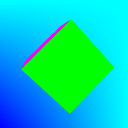
\includegraphics[width=1.05in]{figures/cube_opt/target/110.png}};
        \node (b) [image,right=of a] {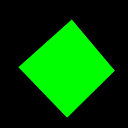
\includegraphics[width=1.05in]{figures/cube_opt/init/110.png}};
        \node (c) [image,right=of b] {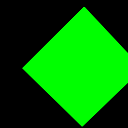
\includegraphics[width=1.05in]{figures/cube_opt/black/110.png}};
        \node (d) [image,right=of c] {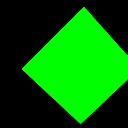
\includegraphics[width=1.05in]{figures/cube_opt/exp/110.png}};
        \node (e) [image,right=of d] {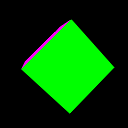
\includegraphics[width=1.05in]{figures/cube_opt/my/110.png}};
        \node (f) [image,right=of e] {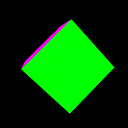
\includegraphics[width=1.05in]{figures/cube_opt/truth/110.png}};

        \node (a) [image,below=of a] {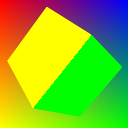
\includegraphics[width=1.05in]{figures/cube_opt/target/118.png}};
        \node (b) [image,right=of a] {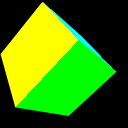
\includegraphics[width=1.05in]{figures/cube_opt/init/118.png}};
        \node (c) [image,right=of b] {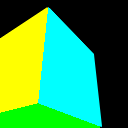
\includegraphics[width=1.05in]{figures/cube_opt/black/118.png}};
        \node (d) [image,right=of c] {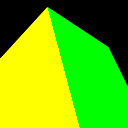
\includegraphics[width=1.05in]{figures/cube_opt/exp/118.png}};
        \node (e) [image,right=of d] {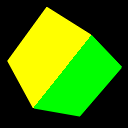
\includegraphics[width=1.05in]{figures/cube_opt/my/118.png}};
        \node (f) [image,right=of e] {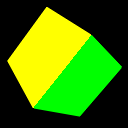
\includegraphics[width=1.05in]{figures/cube_opt/truth/118.png}};

        \small
        \node [below=of a] {(a)目标图像};
        \node [below=of b] {(b)初始化};
        \node [below=of c] {(c)黑色背景};
        \node [below=of d] {(d)数学期望背景};
        \node [below=of e] {(e)本文方法};
        \node [below=of f] {(f)理想背景};
    \end{tikzpicture}
    \caption[立方体的位置和姿态的收敛情况可视化]{
        立方体的位置和姿态的收敛情况可视化。
        (a)立方体渲染于随机背景上的优化目标图像;
        (b)优化前初始化的立方体姿态;
        (c)使用黑色背景模型的优化结果;
        (d)使用随机背景的数学期望作为背景模型的优化结果;
        (e)使用本文方法的优化结果;
        (f)直接使用渲染目标图像时使用的背景的优化结果。
    }
    \label{fig:cube_opt_vis}
\end{figure}
图\ref{fig:cube_opt_vis}可视化了两组实验的结果。
可见若使用不准确的的黑色或数学期望背景模型,则优化过程很容易受到背景中与前景相似的颜色的影响,导致无法正确收敛。
(c)、(d)、(e)对比可以看出越准确的背景模型可产生越好的优化结果,这证实了在一般的可微分渲染应用中,准确的背景模型的必要性。
而利用本章提出的方法即可在不对背景进行建模的情况下,以较高的概率得到准确的结果。

第\ref{chap:recon}章中将介绍将本章方法应用到人脸重建的更多实验。

\section{讨论}
\label{sec:method_discuss}

\paragraph{基于nvdiffrast的实现}
本文基于上文所述理论,基于nvdiffrast\citep{nvdiffrast}中的抗锯齿模块进行了实现。

\begin{figure}
    \centering
    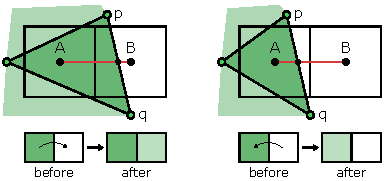
\includegraphics{figures/antialias}
    \caption[nvdiffrast抗锯齿模块的工作流程]{nvdiffrast抗锯齿模块的工作流程\citep{nvdiffrast}。}
    \label{fig:aa}
\end{figure}

为了完整性,这里简要介绍该模块的作用。
如图\ref{fig:aa}所示,该模块修改过的像素为左图的B和右图的A。
其中绿色的部分覆盖该像素的面积占整个像素面积的比例为覆盖率$\sigma$。
记修改前绿色部分的像素值为$\mathbf{c}$,白色背景的像素值为$\mathcal{J}$。
则修改后的像素值为:
\begin{equation}
\mathbf{c}' = \sigma\mathbf{c} + (1-\sigma)\mathcal{J}
\text{。}
\end{equation}

基于该模块,本文使用目标图像$\mathcal{I}$作为背景进行渲染,即$\mathcal{J}=\mathcal{I}$,则公式\ref{eq:loss_n_tilde}中的收缩项可进一步表示为:
\begin{equation}
\sigma\left\| \mathbf{c} - \mathcal{I} \right\|_1 =
\left\| \sigma\mathbf{c} + (1-\sigma)\mathcal{I} - \mathcal{I} \right\|_1 =
\left\| \mathbf{c}' - \mathcal{I} \right\|_1
\text{。}
\label{eq:impl_nvdiffrast}
\end{equation}
如此便可将收缩项中的$\sigma$完全交给该抗锯齿模块处理,且几乎没有额外的计算量。
更好的是,在同一抗锯齿模块中还可以同时处理其他已知背景部分的可见性梯度,例如下巴和脖子间,鼻子和脸颊间。

但nvdiffrast的覆盖率计算是稀疏的,即有部分$\sigma\in(0,1)$的像素无法被检测到,检测的概率和所用3D模型的网格密度有关。
而扩展项的梯度与收缩项相互制衡,因此其梯度的计算必须与收缩项相互耦合,即他们稀疏的模式必须相同
又注意到扩展项的梯度对于边缘的每一个像素是均匀的,因此本实现直接在反向传播时,对所有实际检测到$\sigma\in(0,1)$的像素添加上该项梯度。该方法也基本无额外内存和运算开销。

nvdiffrast的稀疏覆盖率检测有时会导致整体梯度估计的偏差过大,进而导致模型不能收敛到期望的位置,
因此可能还需要手动将相关梯度乘以一个放大系数进行补偿。
下文将对该问题进一步讨论,并提出另一种缓解措施。

\paragraph{L1距离的必要性}
本文中所有的讨论都是基于渲染图像与目标图像的L1距离的,之所以不使用L2或其他距离,主要是基于以下原因:
\begin{itemize}
\item 直接的原因是公式\ref{eq:impl_nvdiffrast}中$\sigma$和求距离的运算的交换需要L1距离。
\item 根本的原因是若将图像看作二维连续函数的离散化,则离散化的操作应尽可能小地对优化造成影响。
使用L1距离才能实现与像素离散化的方式无关的可见性梯度。
如图\ref{fig:problem}c所示,虽然该例子中图像分辨率很低,但其损失函数的梯度仍然是非常平滑的,并未受到像素离散化的影响。
图\ref{fig:l2_loss}展示了另一个使用L2损失的玩具实验的效果。
可见其梯度在像素边缘处出现了明显的阶跃,这是由像素离散化造成的。甚至在像素边缘处得到了为0的梯度,这显然是不合理且不利于优化的。
\end{itemize}

\begin{figure}
    \centering
    \import{build/figures/}{l2_loss.pgf}
    \caption[L2损失与像素离散化相关]{L2损失与像素离散化相关,各图含义参见图\ref{fig:problem}。}
    \label{fig:l2_loss}
\end{figure}

\paragraph{nvdiffrast可见性梯度稀疏的缓解}
前文提到,nvdiffrast的抗锯齿模块计算的覆盖率是稀疏的,即它会错过部分$\sigma\in(0,1)$的像素。
该问题的原因在于其检测渲染图像中不连续性(即包含前景和背景相互遮挡)的方式。
该模块判定相邻两个像素不连续,当且仅当:
\begin{enumerate*}
\item 两个像素渲染自不同的三角形;
\item 其中来自前景的(深度较浅的)三角形在相机视角中处于物体边缘。
\end{enumerate*}
其中,处于边缘的判定方法为:来自前景的三角形满足以下条件之一:
\begin{enumerate*}
\item 在背景方向上无与其相邻的三角形;
\item 在背景方向上与其相邻的三角形朝向相机背面。
\end{enumerate*}
然而,真正处于边缘的三角形可能并未被渲染图像的任何一个像素采样到。
处于边缘的三角形被采样到的概率正比于其在渲染图像上的投影面积。
但为了提升精度而使用更高密度的网格会导致每个三角形面积的下降;
更雪上加霜的是,位于边缘的三角形的法向通常与相机方向夹角很大,导致其在渲染图像上的投影面积更小。
最终导致即使使用很高的分辨率也无法实现令人满意的采样概率。

为缓解该问题,本文提出放松处于边缘的判定条件,添加一条:背景未被任何三角形覆盖。
在该条件下即可保证与未知背景交界的所有边缘均被检测到。
但付出的代价是部分梯度不能正确地传递到真正处于边缘的顶点上,
而是被传递到与边缘相近的真正被采样到的三角形的顶点上。
但是在完整的优化问题中通常都具有鼓励模型局部光滑的正则项,这些梯度的影响最终将被较为均匀地分布到更大的区域上,因此这些偏差应该不会造成太大的影响。
图\ref{fig:vis_grad}展示了一些具体的例子。

此外,该方法只能缓解模型与未知背景间的不连续性判定,而对模型自身不同部分的遮挡无能为力。
这会导致内部的可见性梯度偏小,从而导致整体梯度估计发生偏差。
其具体影响需根据实际应用进一步分析。

\begin{figure}
    \centering
    \begin{subfigure}{0.33\textwidth}
        \centering
        \begin{tikzpicture}
            \path[use as bounding box] (-0.5,-0.5) rectangle (4,2.5);
            \draw [help lines] (0,0) grid [step=2cm] (4,2);
            \draw[red, name path=H] (1,1) -- (3,1);
            \filldraw (1,1) circle (1pt) node [above] {A}
                      (3,1) circle (1pt) node [above] {B};

            \coordinate [label=right:p] (p) at (1.2,2.2);
            \coordinate [label=right:q] (q) at (2,-0.3);
            \coordinate (r) at (-0.5,1);

            \draw (p) -- (r) -- (q);
            \draw [green!30!black, name path=T, thick] (p) -- (q);
            \path [name intersections={of=H and T,by=I}];

            \draw[fill=green] (p) circle (2pt);
            \draw[fill=green] (q) circle (2pt);
            \draw[fill] (I) circle (1pt);

            \begin{pgfonlayer}{background}
                \fill[green!50] (p) -- (1.1, 2.5) -- (-0.5,2.5) -- (-0.5,-0.3) --  (-0.5,-0.5) -- (2, -0.5) -- (q);
                \fill[green!80!black] (p) -- (q) -- (r) -- cycle;
            \end{pgfonlayer}
        \end{tikzpicture}
        \caption{正常检测到的边缘}
    \end{subfigure}%
    \begin{subfigure}{0.33\textwidth}
        \centering
        \begin{tikzpicture}
            \path[use as bounding box] (-0.5,-0.5) rectangle (4,2.5);
            \draw [help lines] (0,0) grid [step=2cm] (4,2);
            \draw[red, name path=H] (1,1) -- (3,1);
            \filldraw (1,1) circle (1pt) node [above] {A}
                      (3,1) circle (1pt) node [above] {B};

            \coordinate [label=above:p] (p) at (1.2,2.2);
            \coordinate [label=below:q] (q) at (2,-0.3);
            \coordinate (r) at (-0.5,1);
            \coordinate (s) at (2.2,2.2);
            \coordinate (t) at (2.6,-0.3);

            \draw (p) -- (r) -- (q);
            \draw (s) -- (t) -- (q) -- cycle;
            \draw (s) -- (p);
            \draw [green!30!black, name path=T, thick] (p) -- (q);
            \path [name intersections={of=H and T,by=I}];

            \draw[fill=red] (p) circle (2pt);
            \draw[fill=red] (q) circle (2pt);
            \draw[fill=gray!50] (s) circle (2pt);
            \draw[fill=gray!50] (t) circle (2pt);
            \draw[fill] (I) circle (1pt);

            \begin{pgfonlayer}{background}
                \fill[green!50] (s) -- (2.1, 2.5) -- (-0.5,2.5) -- (-0.5,-0.3) --  (-0.5,-0.5) -- (2.6, -0.5) -- (t);
                \fill[green!80!black] (p) -- (q) -- (r) -- cycle;
            \end{pgfonlayer}
        \end{tikzpicture}
        \caption{缓解情况1}
    \end{subfigure}%
    \begin{subfigure}{0.33\textwidth}
        \centering
        \begin{tikzpicture}
            \path[use as bounding box] (-0.5,-0.5) rectangle (4,2.5);
            \draw [help lines] (0,0) grid [step=2cm] (4,2);
            \draw[red, name path=H] (1,1) -- (3,1);
            \filldraw (1,1) circle (1pt) node [above] {A}
                      (3,1) circle (1pt) node [above] {B};

            \coordinate [label=above:p] (p) at (0.6,2.2);
            \coordinate [label=right:q] (q) at (2.2,-0.3);
            \coordinate (r) at (0.5,-0.2);
            \coordinate (s) at (2.2,2.2);

            \draw (p) -- (r) -- (q);
            \draw (q) -- (s) -- (p);
            \draw [green!30!black, name path=T, thick] (p) -- (q);
            \path [name intersections={of=H and T,by=I}];

            \draw[fill=red] (p) circle (2pt);
            \draw[fill=green] (q) circle (2pt);
            \draw[fill=gray!50] (s) circle (2pt);
            \draw[fill] (I) circle (1pt);

            \begin{pgfonlayer}{background}
                \fill[green!50] (s) -- (2.1, 2.5) -- (-0.5,2.5) -- (-0.5,-0.3) --  (-0.5,-0.5) -- (2.2, -0.5) -- (q);
                \fill[green!80!black] (p) -- (q) -- (r) -- cycle;
            \end{pgfonlayer}
        \end{tikzpicture}
        \caption{缓解情况2}
    \end{subfigure}
    \caption[nvdiffrast可见性梯度稀疏的原因及其缓解方法]{nvdiffrast可见性梯度稀疏的原因及其缓解方法。
    (a)展示了可正常检测到可见性梯度的情况,即A像素的采样点正好落在处于边缘的三角形上。其中绿色顶点表示梯度正确传递的顶点。
    (b)、(c)展示了两种常见的检测失败的情况,灰色顶点表示本应获得可见性梯度却未获得的顶点。
    (b)情况常见于脸颊与背景间,相机视线与表面法线夹角大,每个三角形的投影面积被大幅压缩,导致被采样到的概率减小。
    (c)情况常见于模型被裁剪的边缘,部分三角形与模型仅有一个点连接,这些三角形有较高概率被A像素采样,却不被识别为处于边缘。
    本文提出的方法能在B像素采样到背景时,通过将本应传给灰色顶点的可见性梯度转而传递给红色像素,从而缓解该问题。}
    \label{fig:vis_grad}
\end{figure}

\paragraph{局限性}

虽然本章提出的方法能在一定程度上解决在未知背景时的逆渲染问题,但该方法仍然不如直接采集真实的背景图像,并对整张图片应用常规可微分渲染方法好。
本章方法中的超参数$\alpha$的选择与模型拟合误差的分布有关,如果拟合误差在空间上分布非常不均匀,或前景与背景差别过小则可能无法找到合适的参数。
此外,失焦造成的边缘模糊,以及碰巧背景颜色与人脸较为相近的情况下,本算法的对齐质量也会下降。

因此,如采用三脚架拍摄时,则应该尽量在拍摄的同时采集背景,即保持相机位置和拍摄参数不变,分别拍摄有人在画面中的和仅有背景的照片。

\section*{本章小结}

本章提出了一种可适应未知背景的可微分逆渲染方法,该方法能够在无需对背景建模的境况下,将前景模型(如人脸)拟合到目标图像中。
本章首先将图像视为连续函数,并在提出了一种面积归一化的像素损失函数,并在一维情况下对其进行了分析,说明了其可以有效帮助模型对齐到期望的边缘。
随后本章将损失函数推广到离散到像素的图像上,并进一步分析了其梯度,将梯度分为收缩和扩展两项,说明了推广后的损失函数的作用机理。
在此基础上,利用了其梯度仅在模型与背景交界处不为0的特点,本章提出了一种更高效的实现方式:在nvdiffrast的抗锯齿模块的基础上,在几乎不增加额外计算和存储开销的情况下实现了本章所述方法。
最后通过实验验证了本章提出的方法确实能实现在未知背景下的逆渲染。

第\ref{chap:recon}章将介绍如何把本章方法应用到人脸重建中。
此外,该方法在多视角或多帧视频输入的重建中的应用还有待探索。
更多的信息带来的更强的正则化可能使得本方法更加鲁棒;但这些信息本身就能提供边缘对齐的额外的线索,可能导致本方法的必要性降低。
